\documentclass{report}
\usepackage{graphicx}
\usepackage{pgfplots}
\begin{document}
\begin{titlepage}
\centering
{\bfseries\LARGE Instituto Tecnol\'ogico de Costa Rica \par}
\vspace{1cm}
{\scshape\Large Facultad de Ingenier\'ia en Computaci\'on \par}
\vspace{3cm}
{\scshape\Huge Simulaci\'on de propagaci\'on \\
de COVID-19\par}
\vspace{3cm}
{\itshape\Large Proyecto 2\par}
\vfill
{\Large Emanuelle Jim\'enez S.\par}
{\Large Fabrizio Alvarado B\par}
\vfill
{\Large Junio 2020 \par}
\end{titlepage}
\newpage
\section{Gr\'afico}
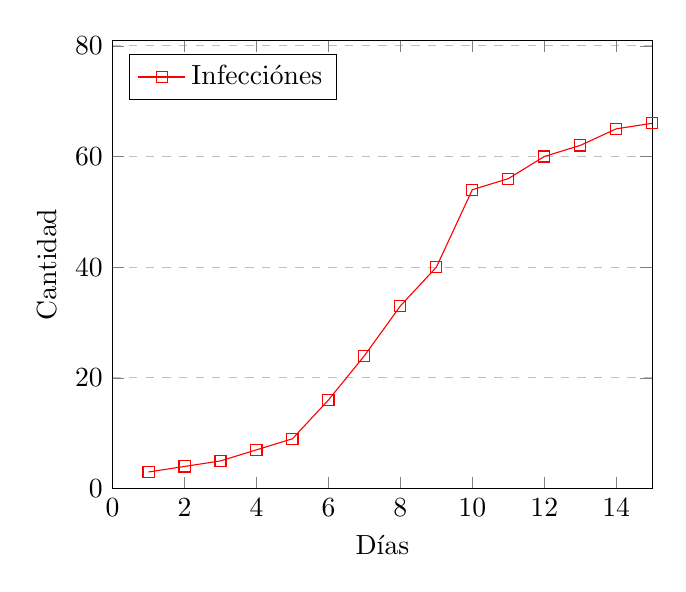
\begin{tikzpicture}
\begin{axis}[
xlabel={D\'ias},
ylabel={Cantidad},
xmin=0, xmax=15,
ymin=0, ymax=81,
legend pos=north west,
ymajorgrids=true,
grid style=dashed,
]
\addplot[
color=red,
mark=square,
]
coordinates {
(1, 3)(2, 4)(3, 5)(4, 7)(5, 9)(6, 16)(7, 24)(8, 33)(9, 40)(10, 54)(11, 56)(12, 60)(13, 62)(14, 65)(15, 66)
};
\legend{Infecci\'ones}
\end{axis}
\end{tikzpicture}
\newpage
\section{Cambios en el mapa}
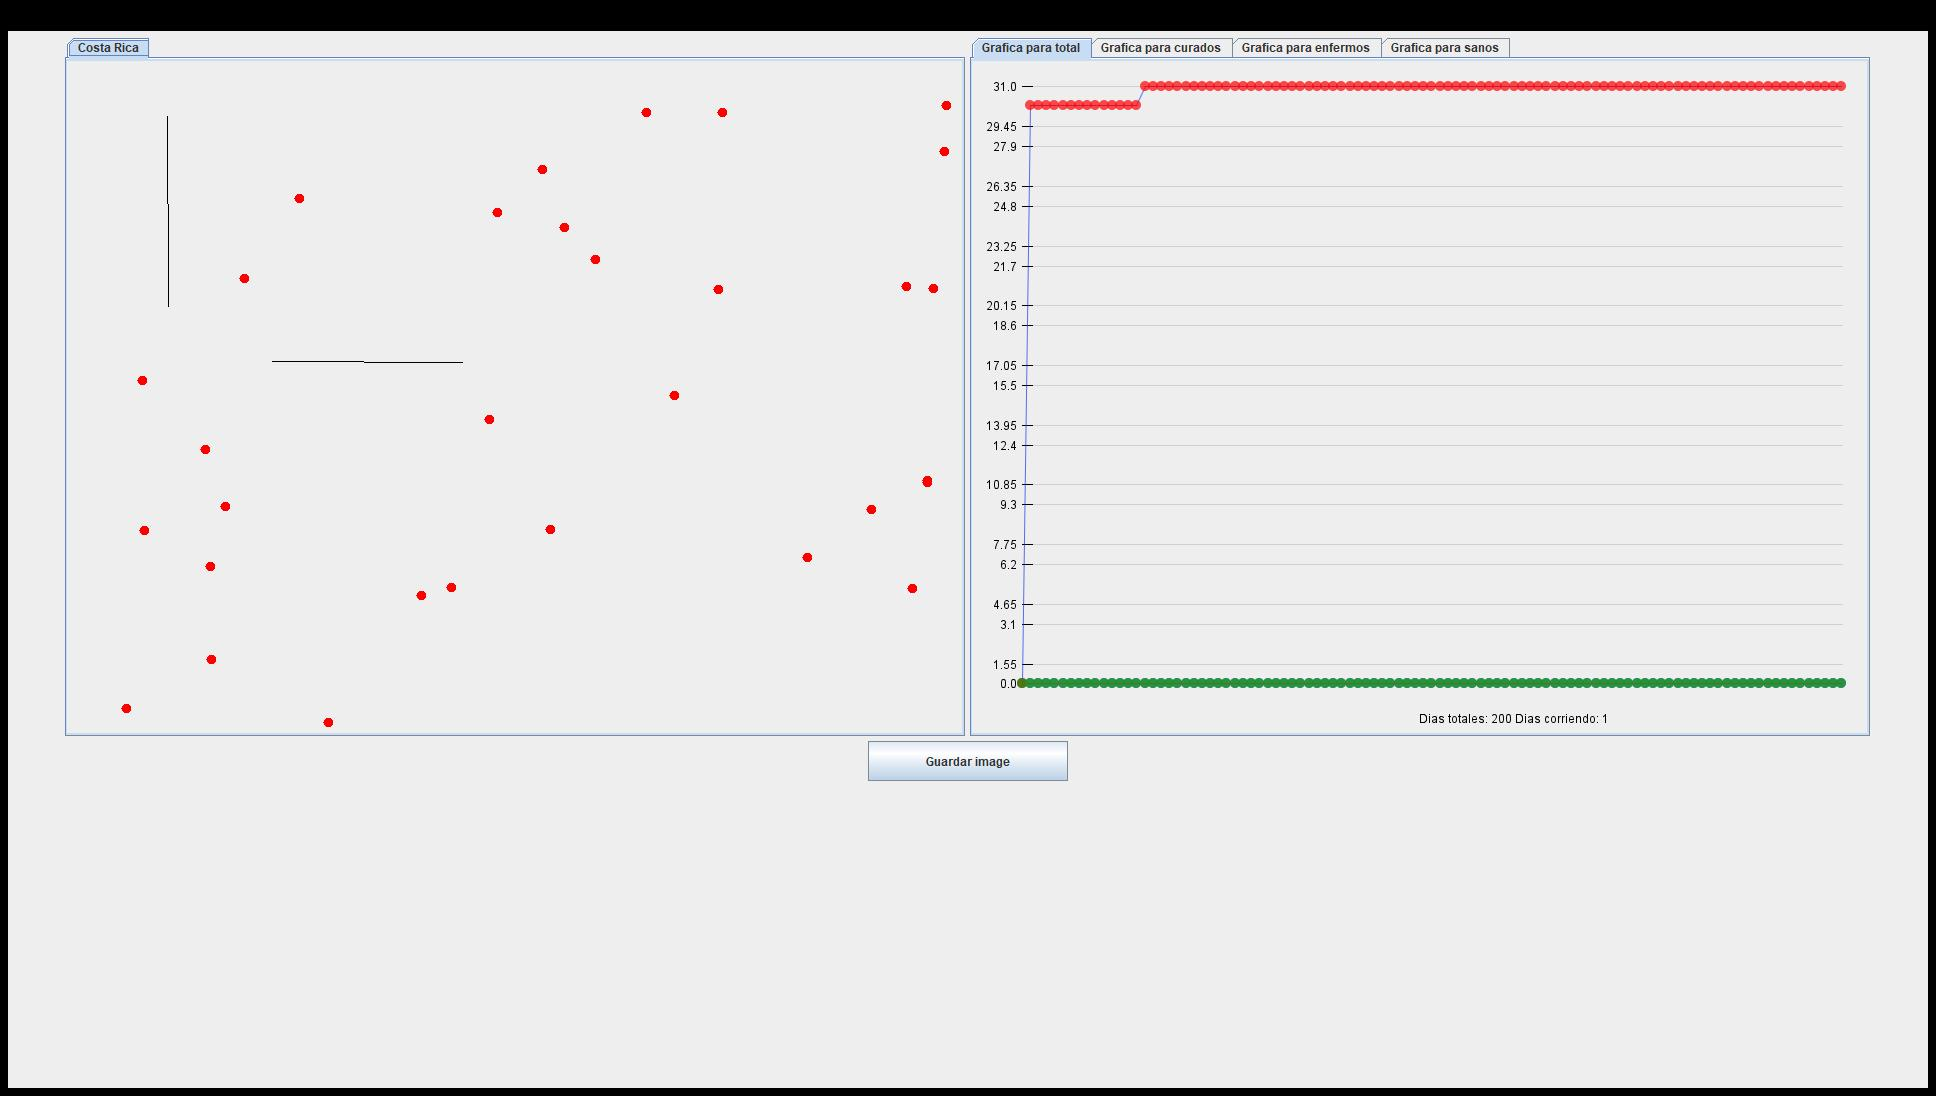
\includegraphics[scale=0.20]{1}
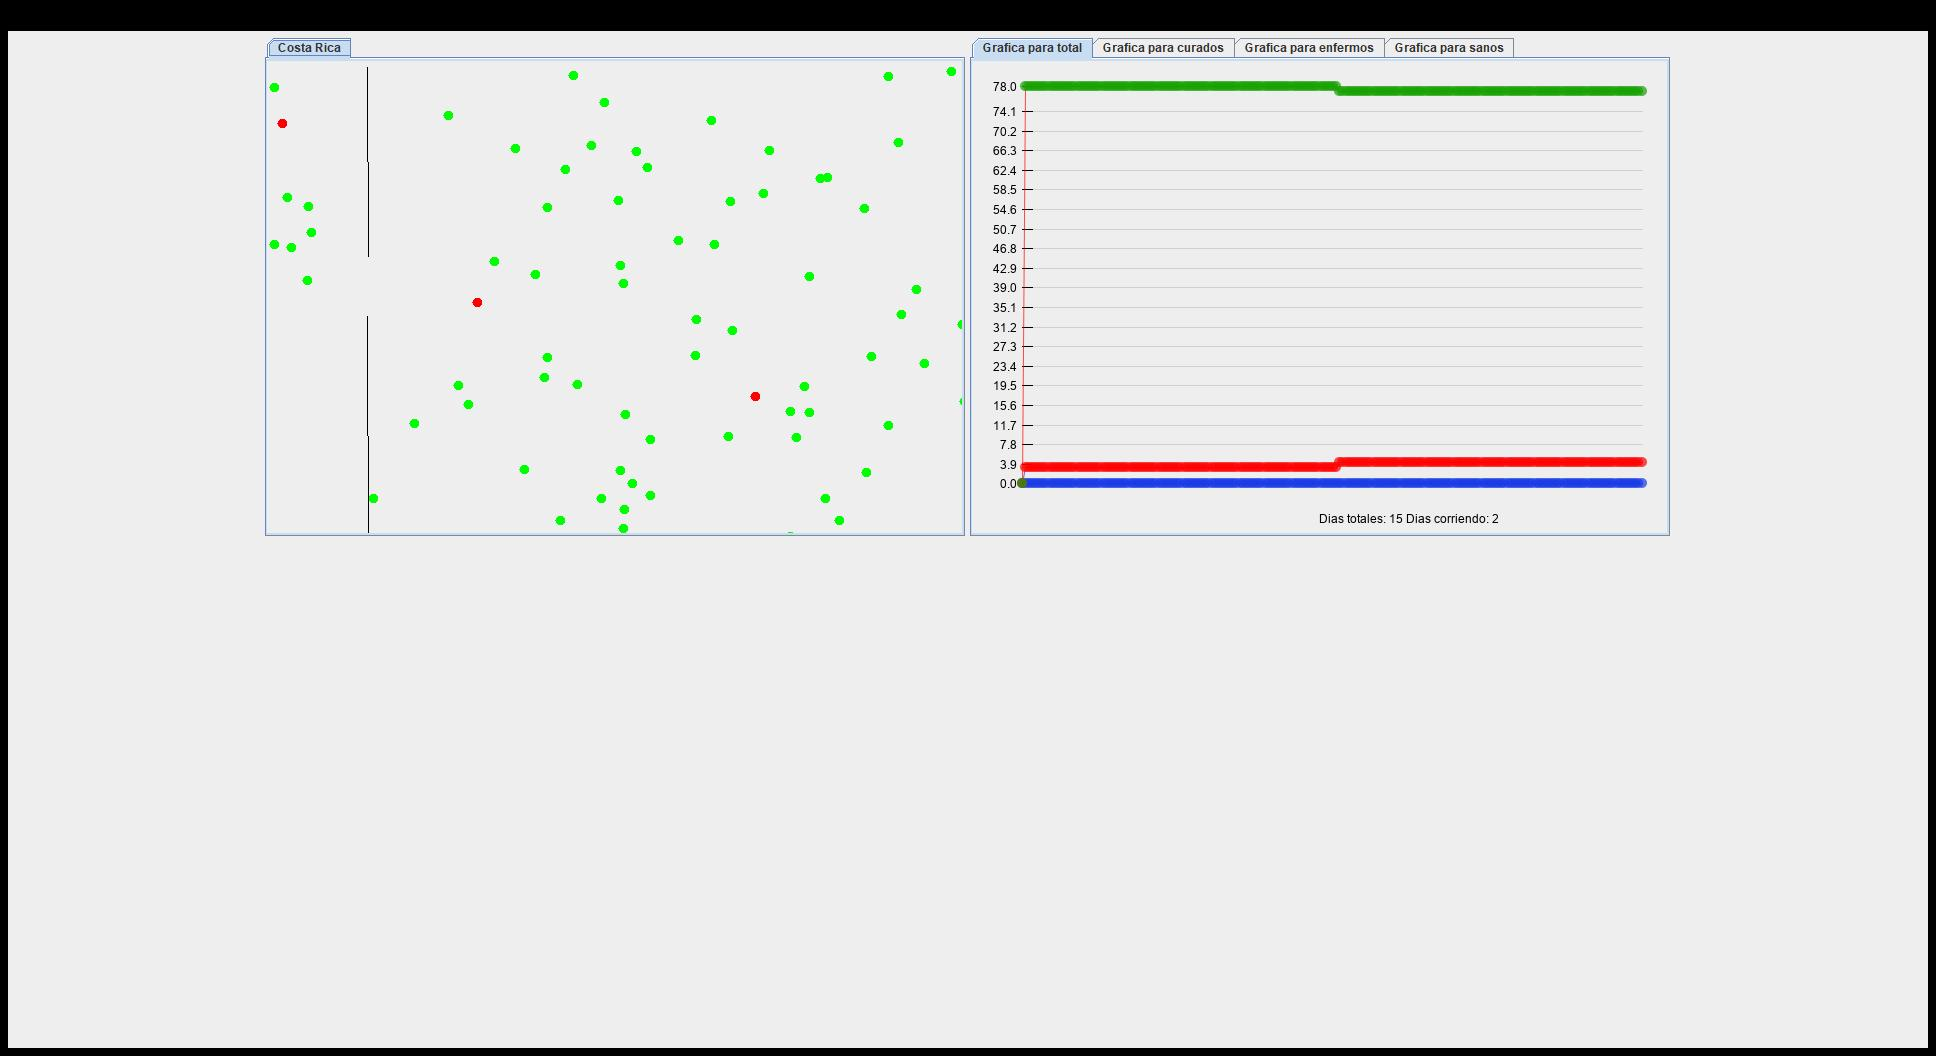
\includegraphics[scale=0.20]{2}
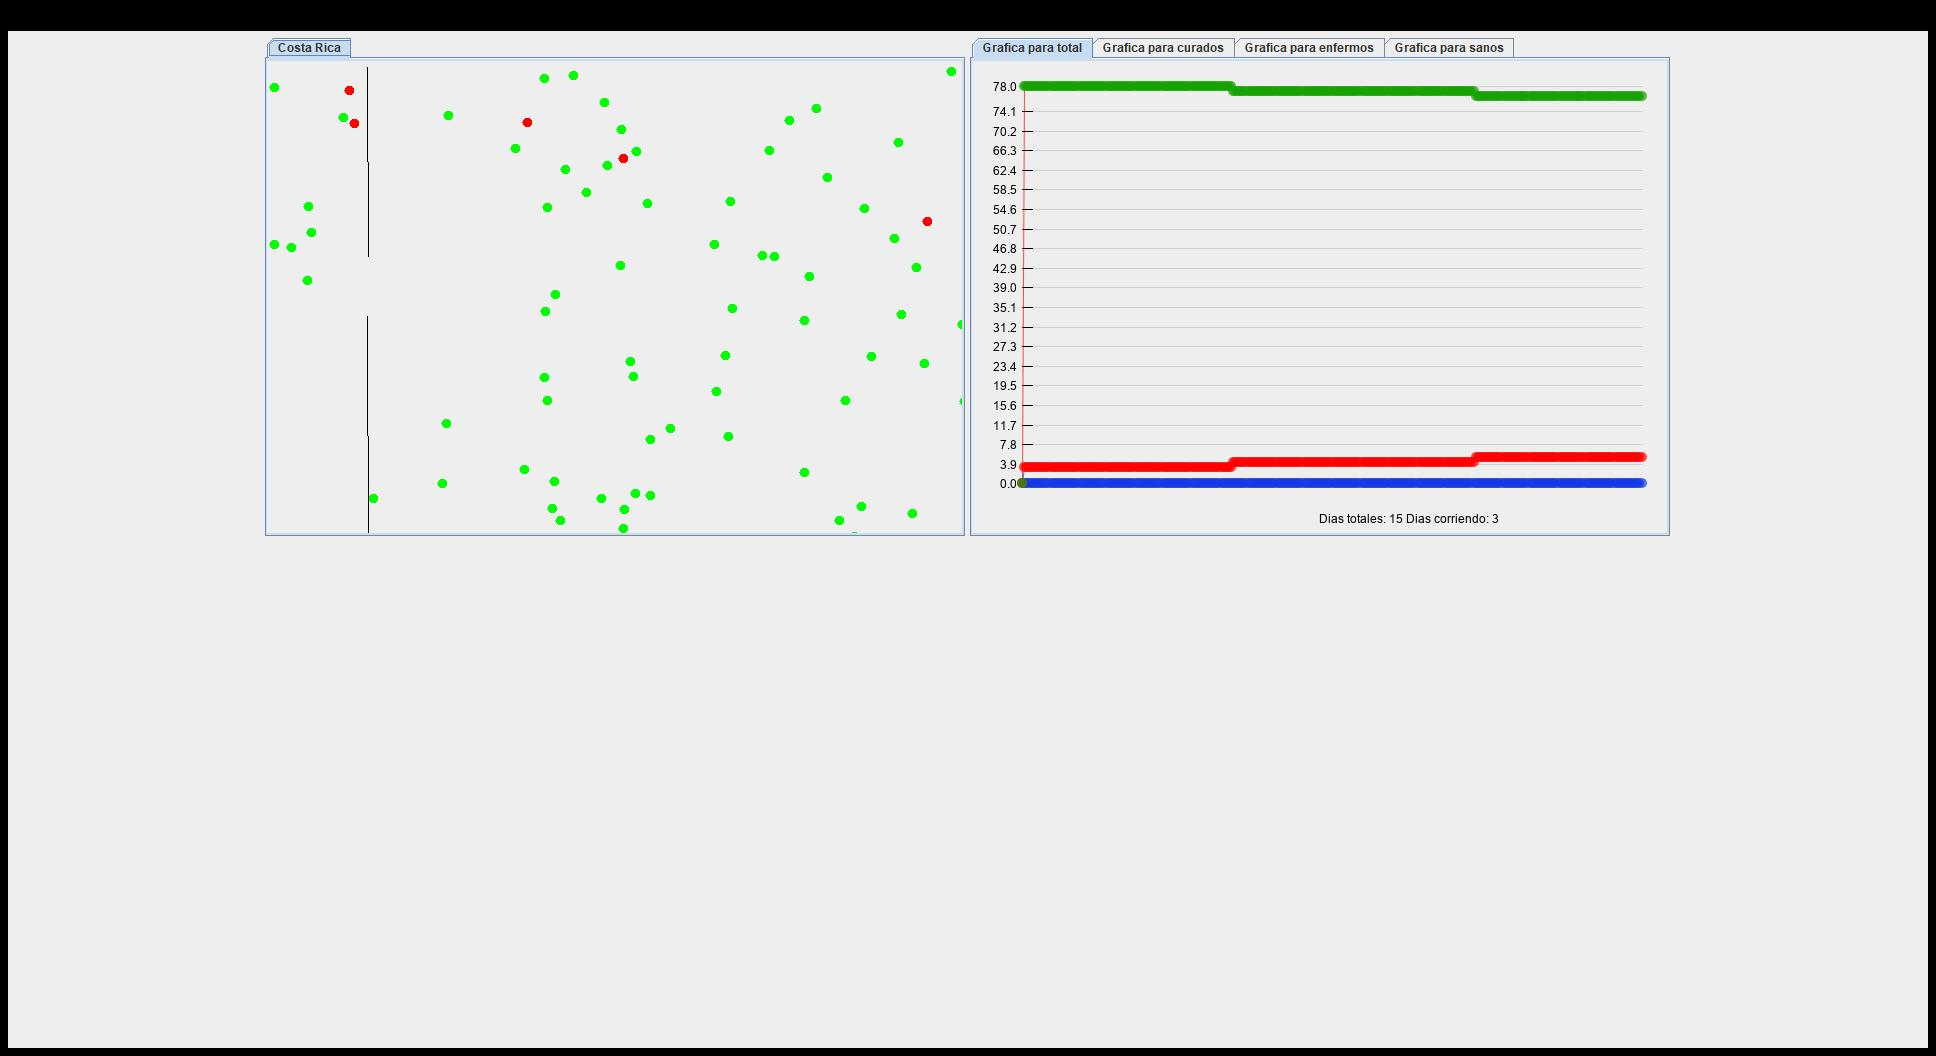
\includegraphics[scale=0.20]{3}
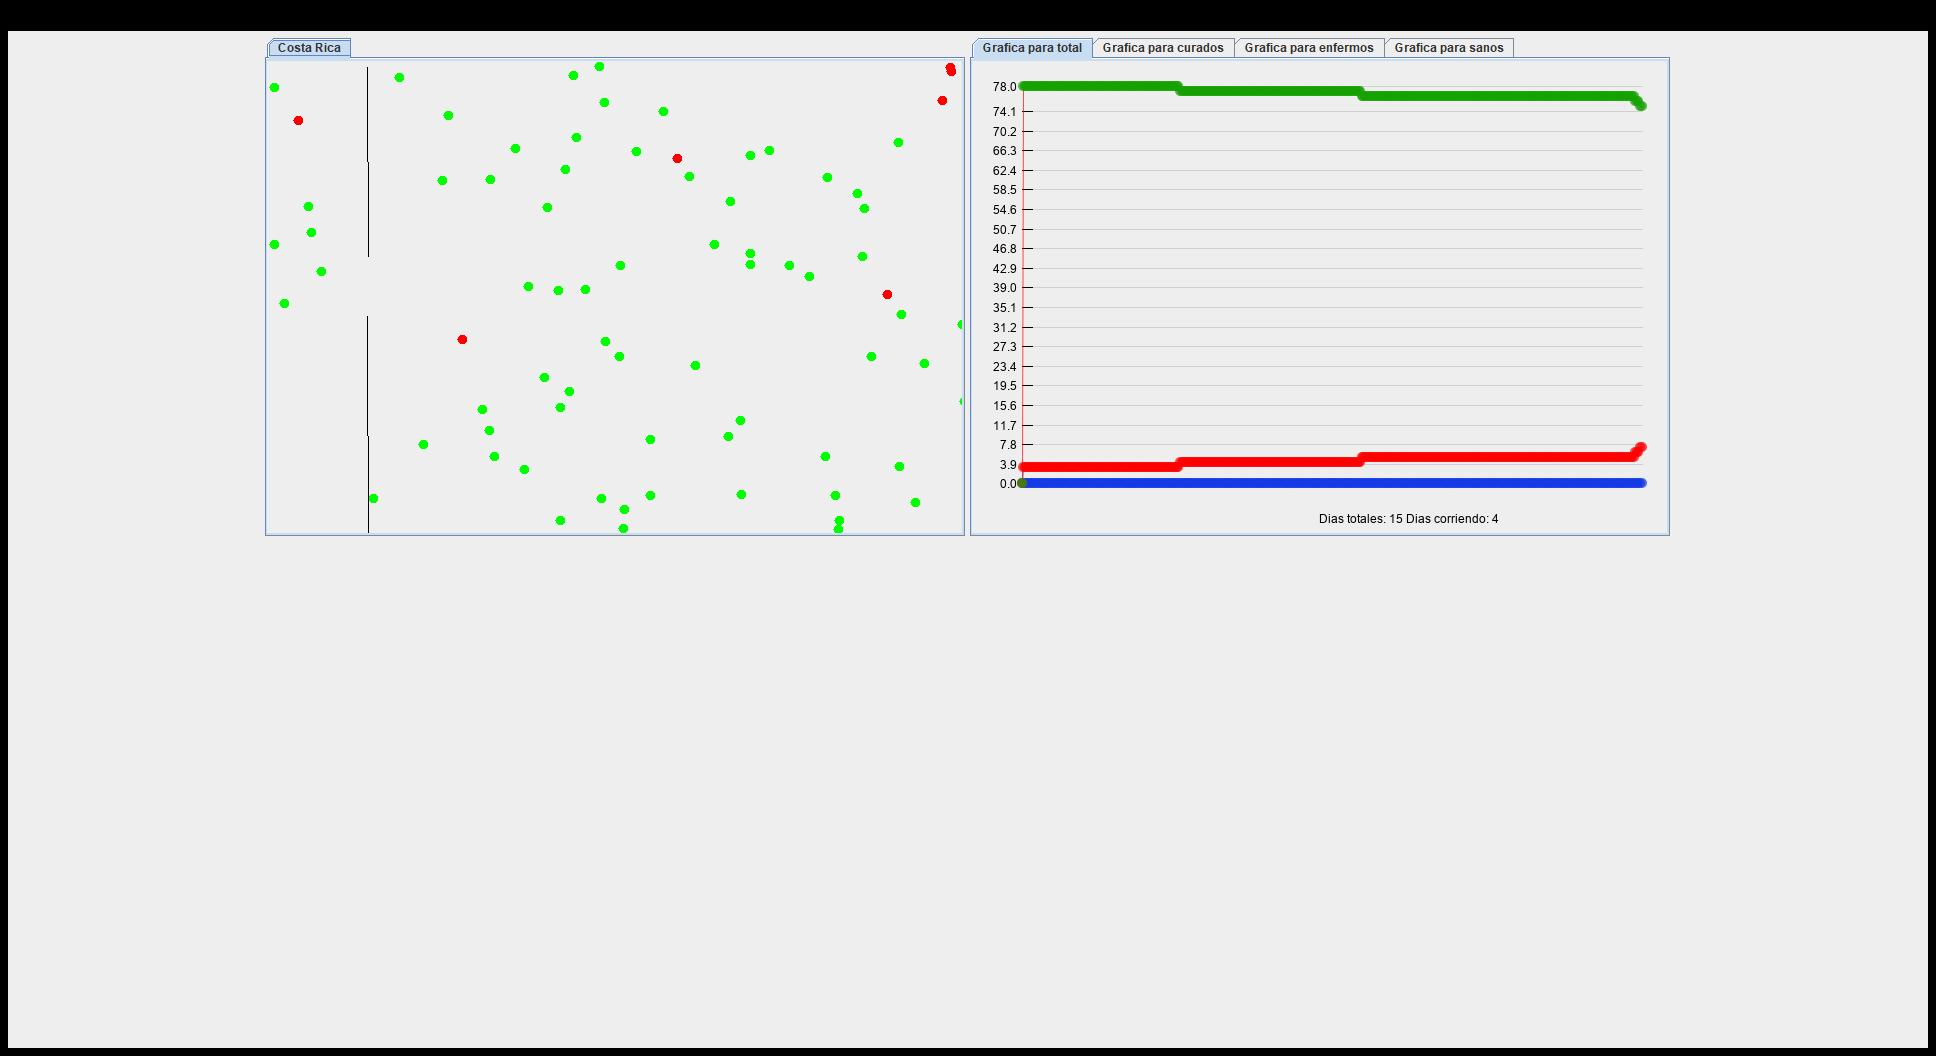
\includegraphics[scale=0.20]{4}
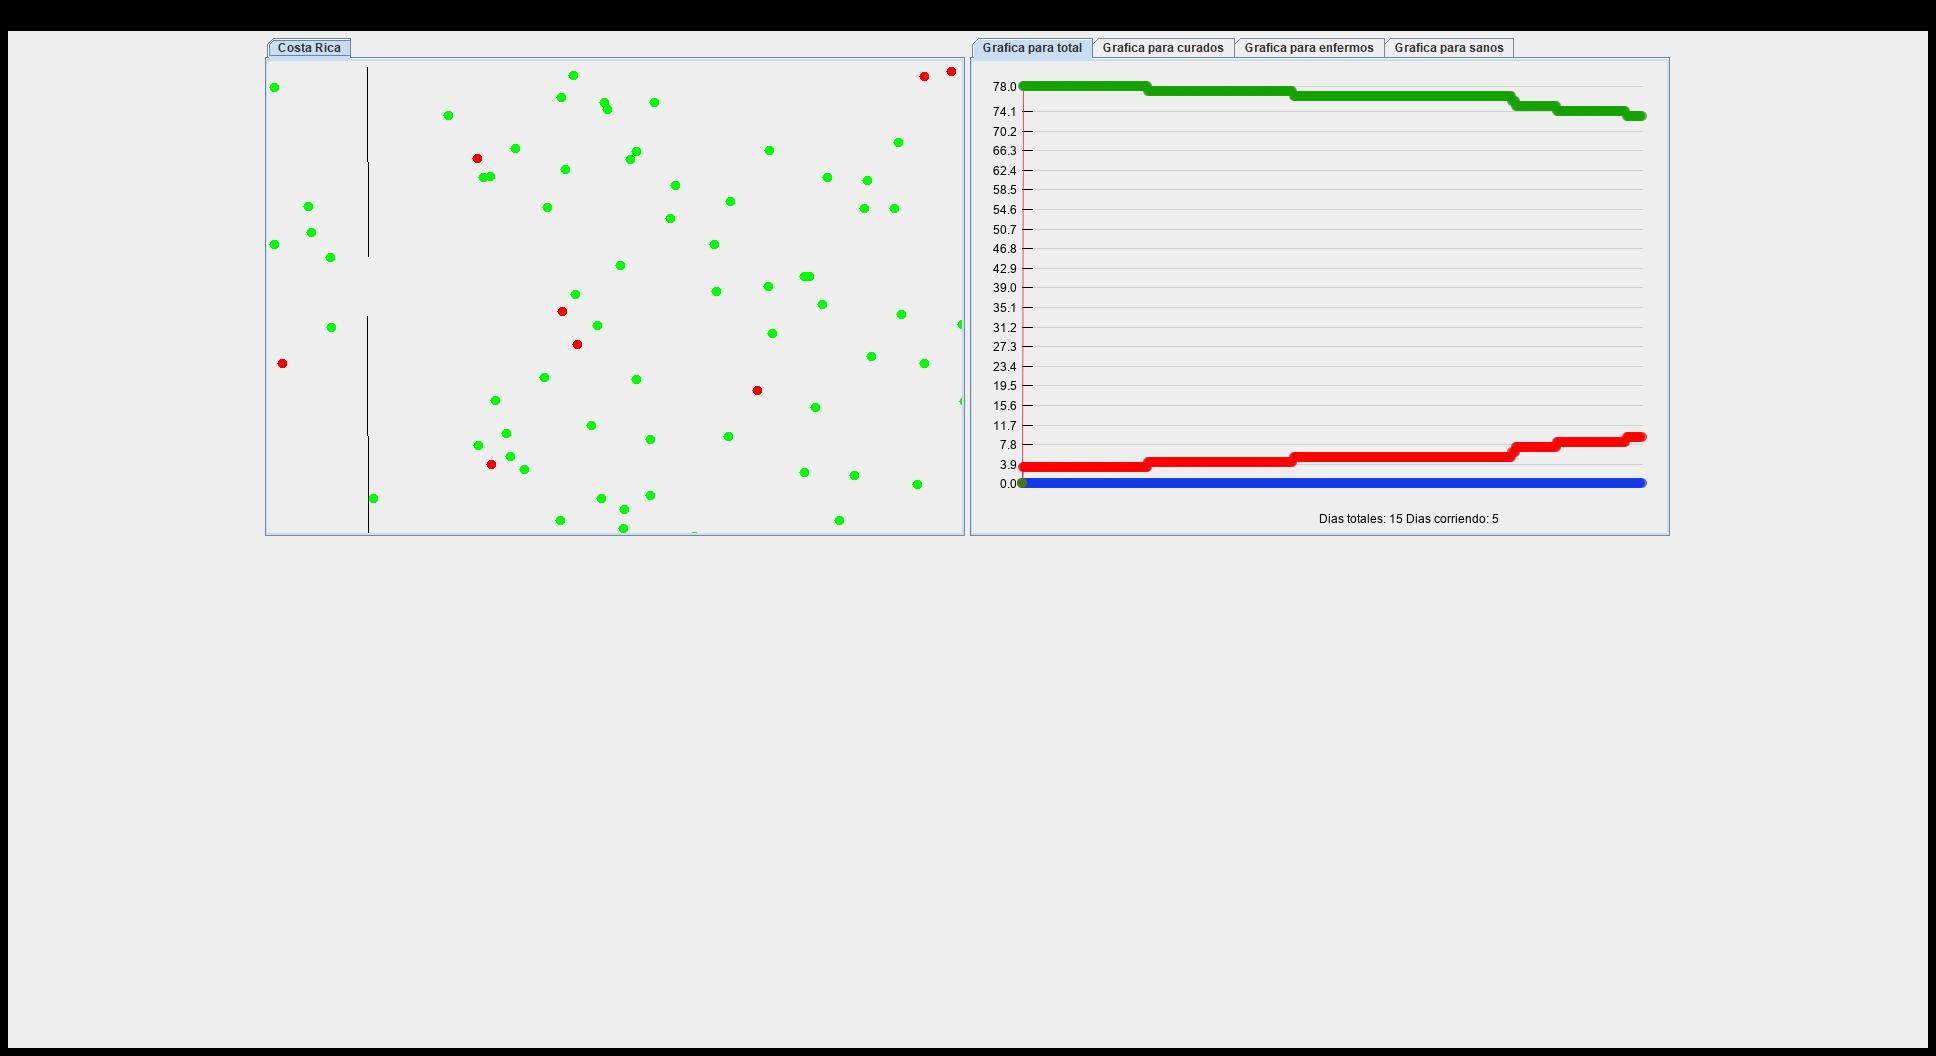
\includegraphics[scale=0.20]{5}
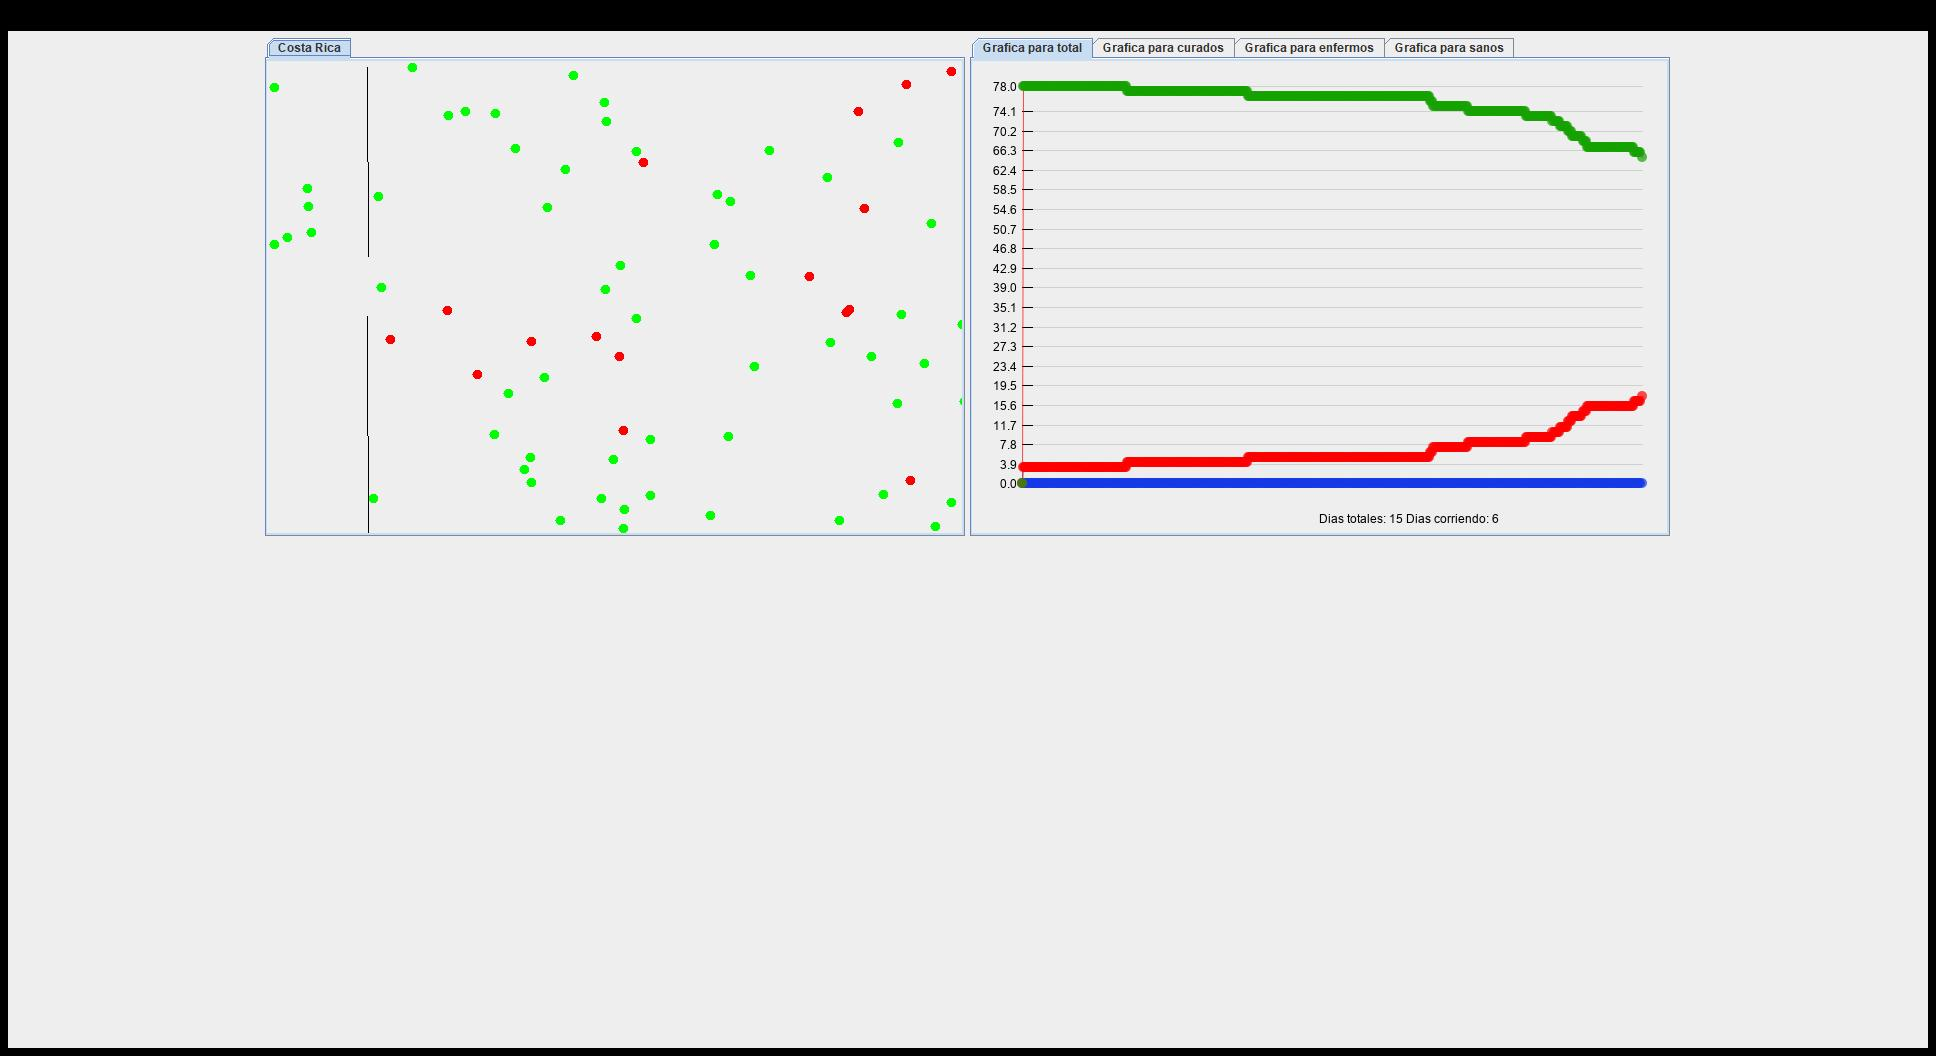
\includegraphics[scale=0.20]{6}
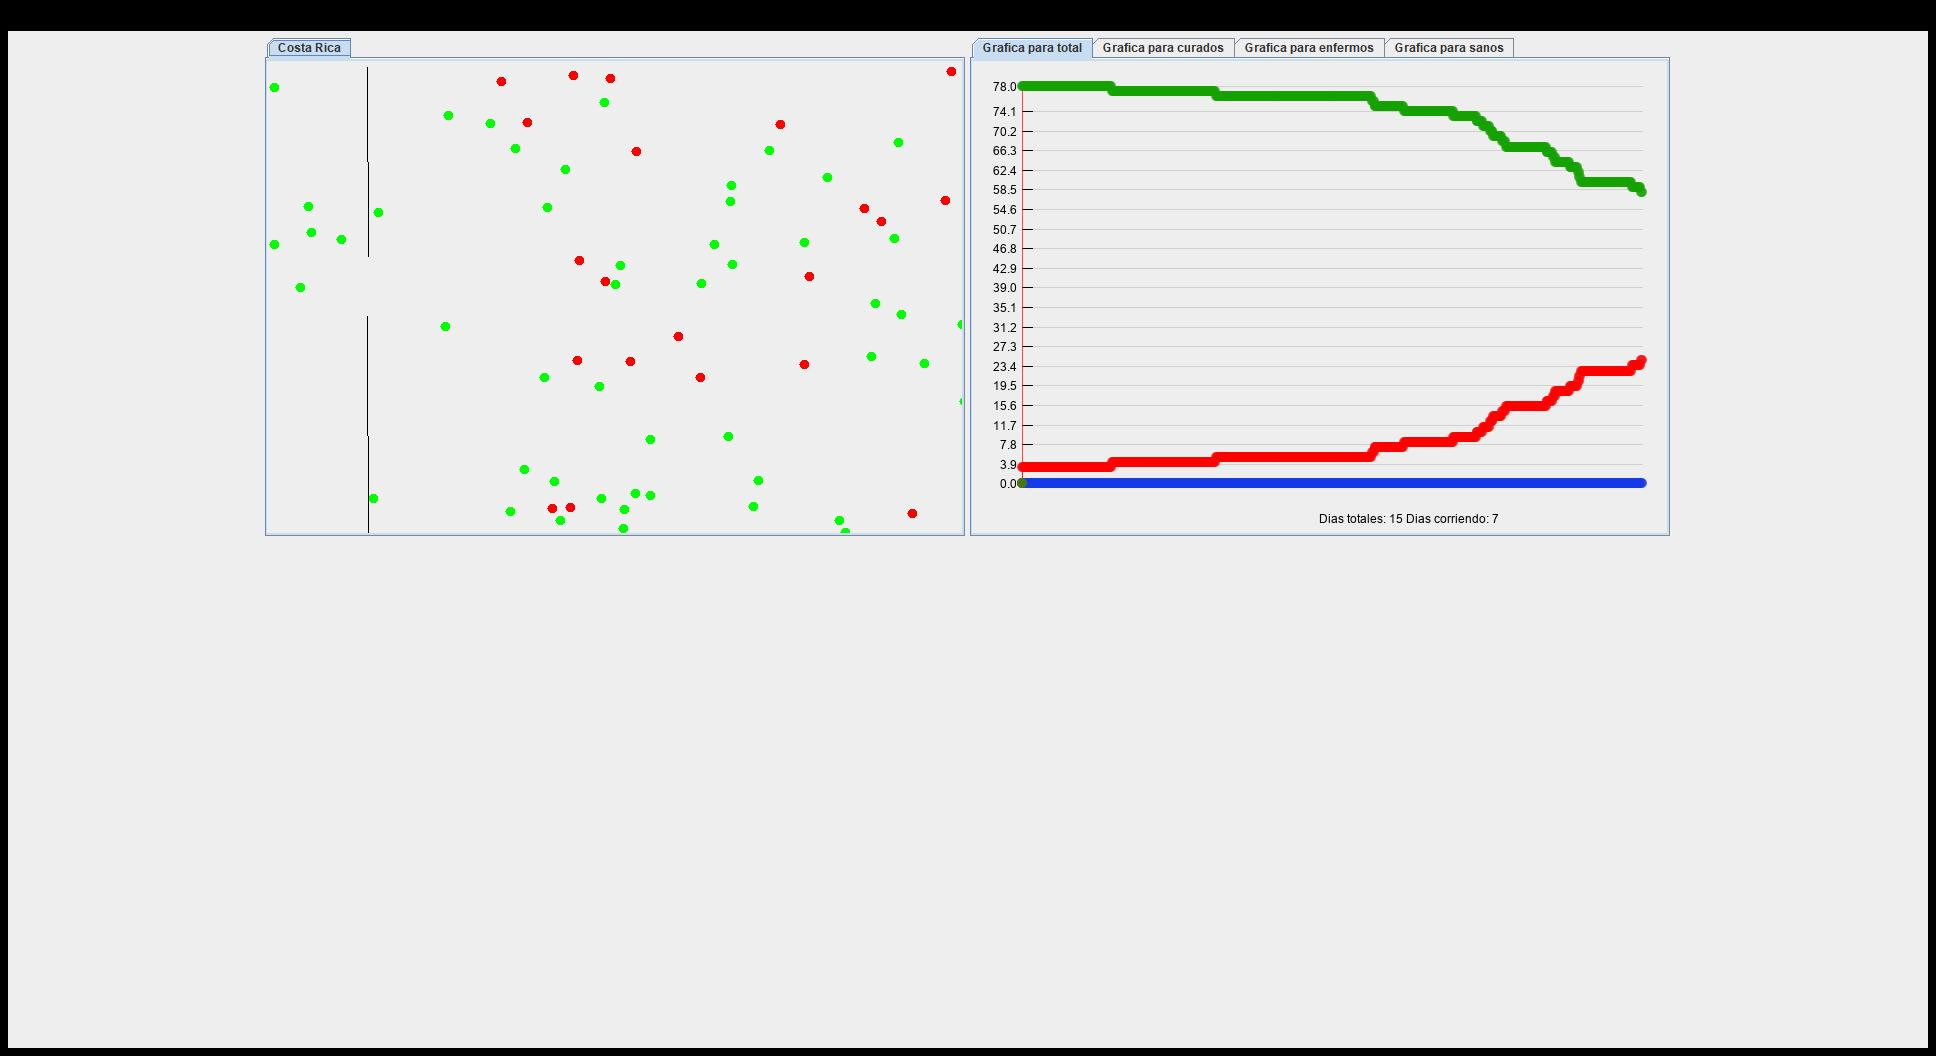
\includegraphics[scale=0.20]{7}
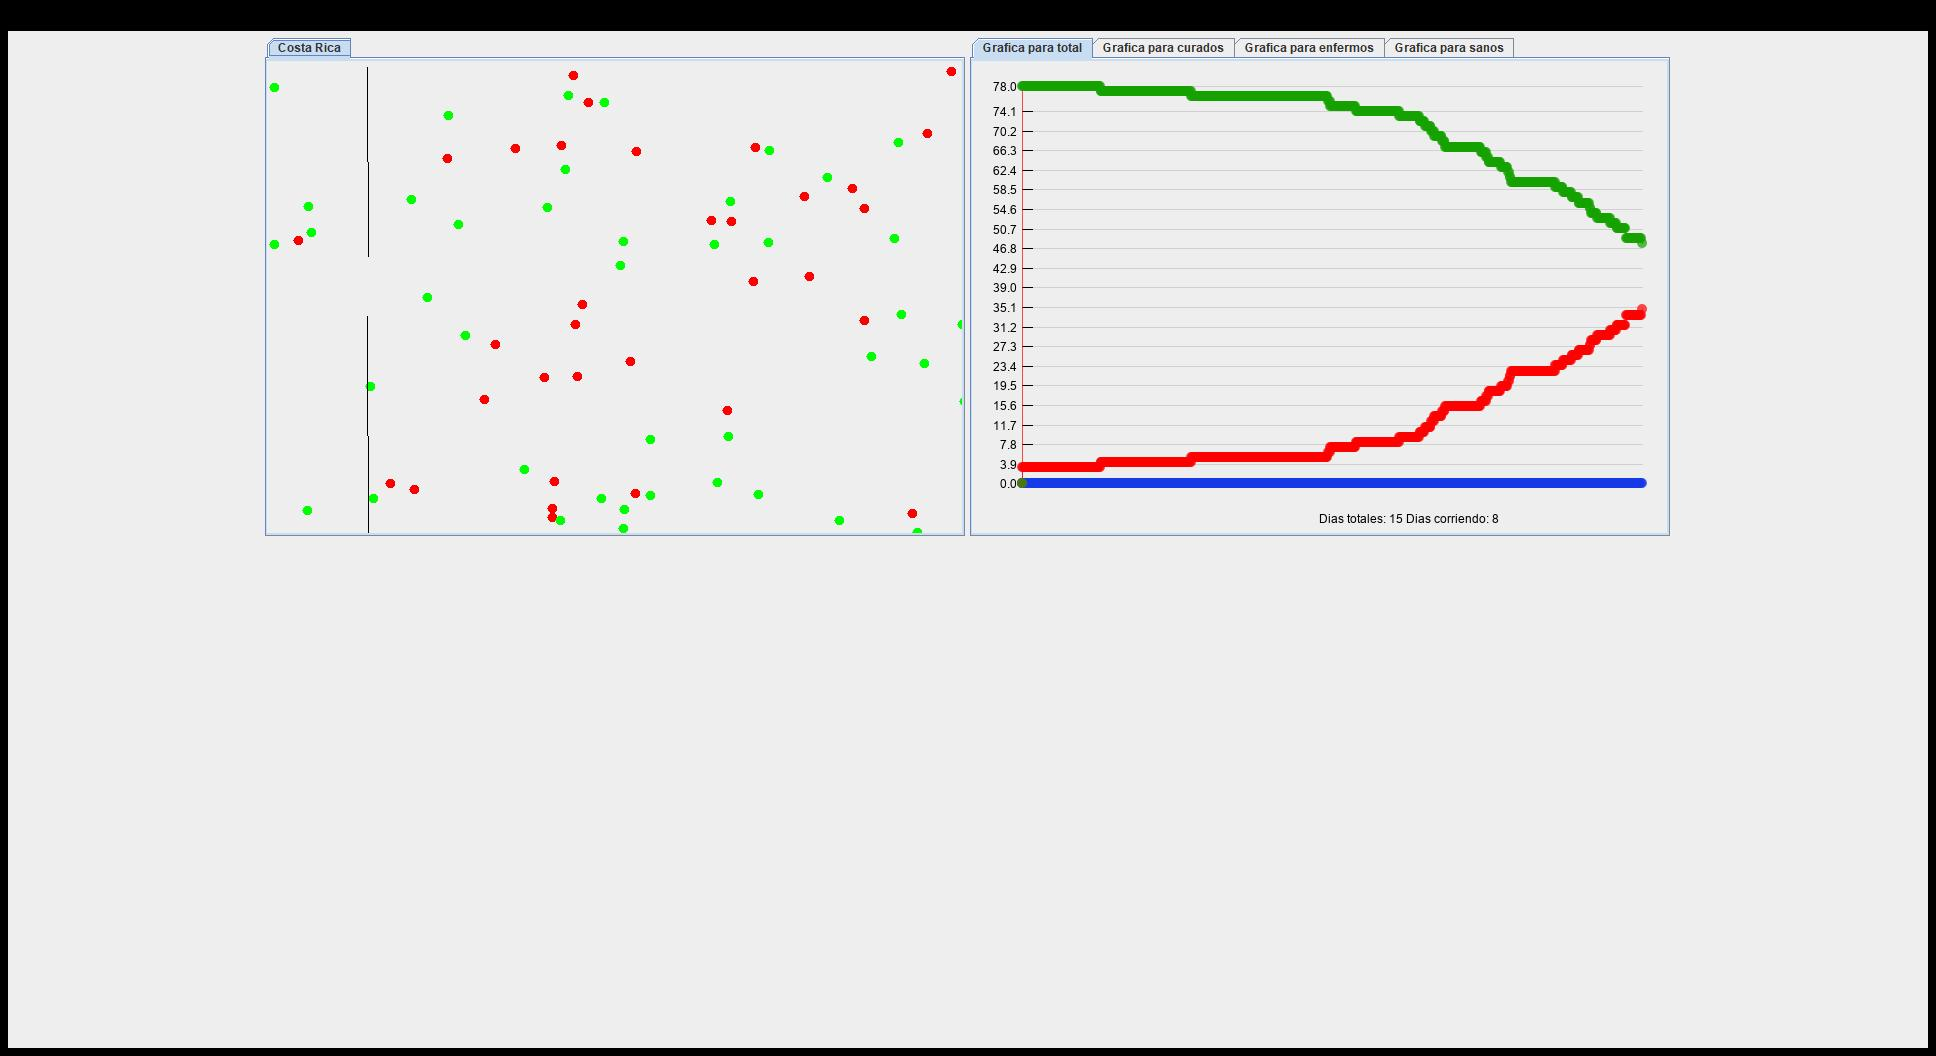
\includegraphics[scale=0.20]{8}
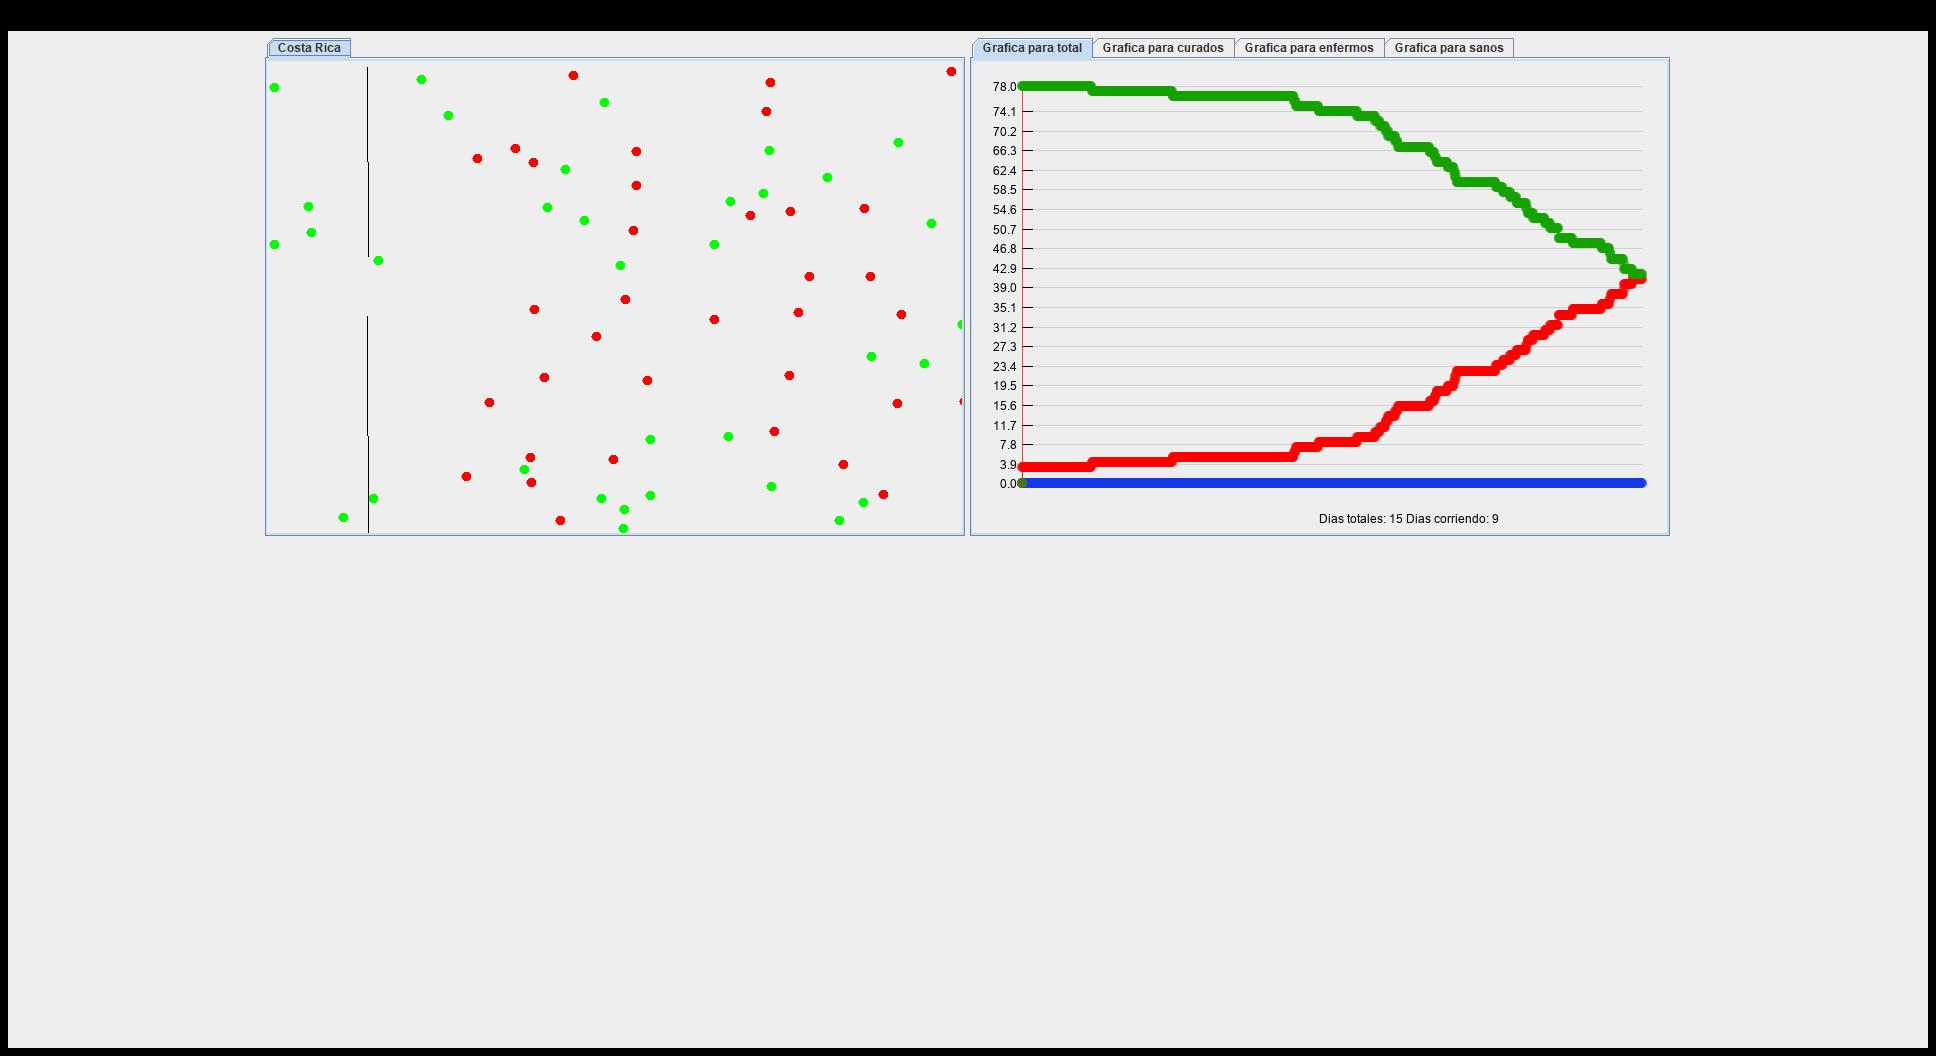
\includegraphics[scale=0.20]{9}
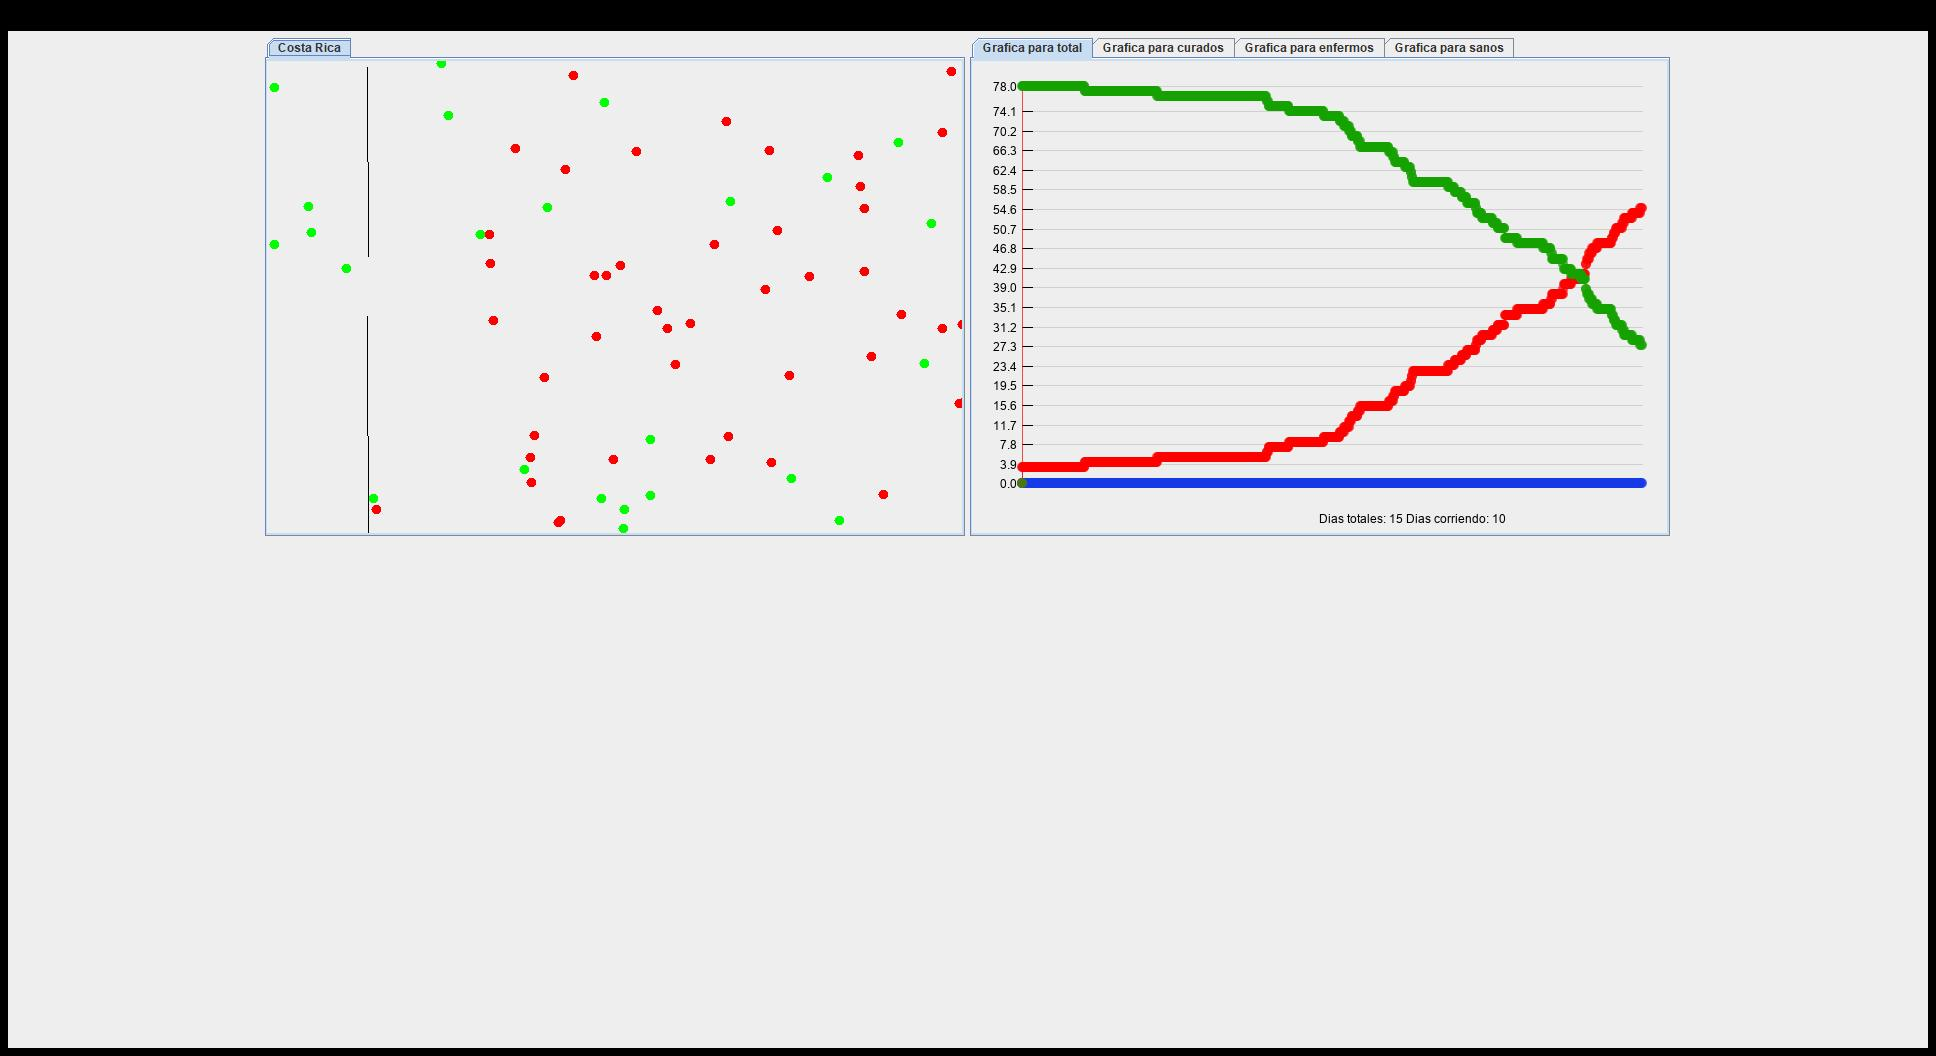
\includegraphics[scale=0.20]{10}
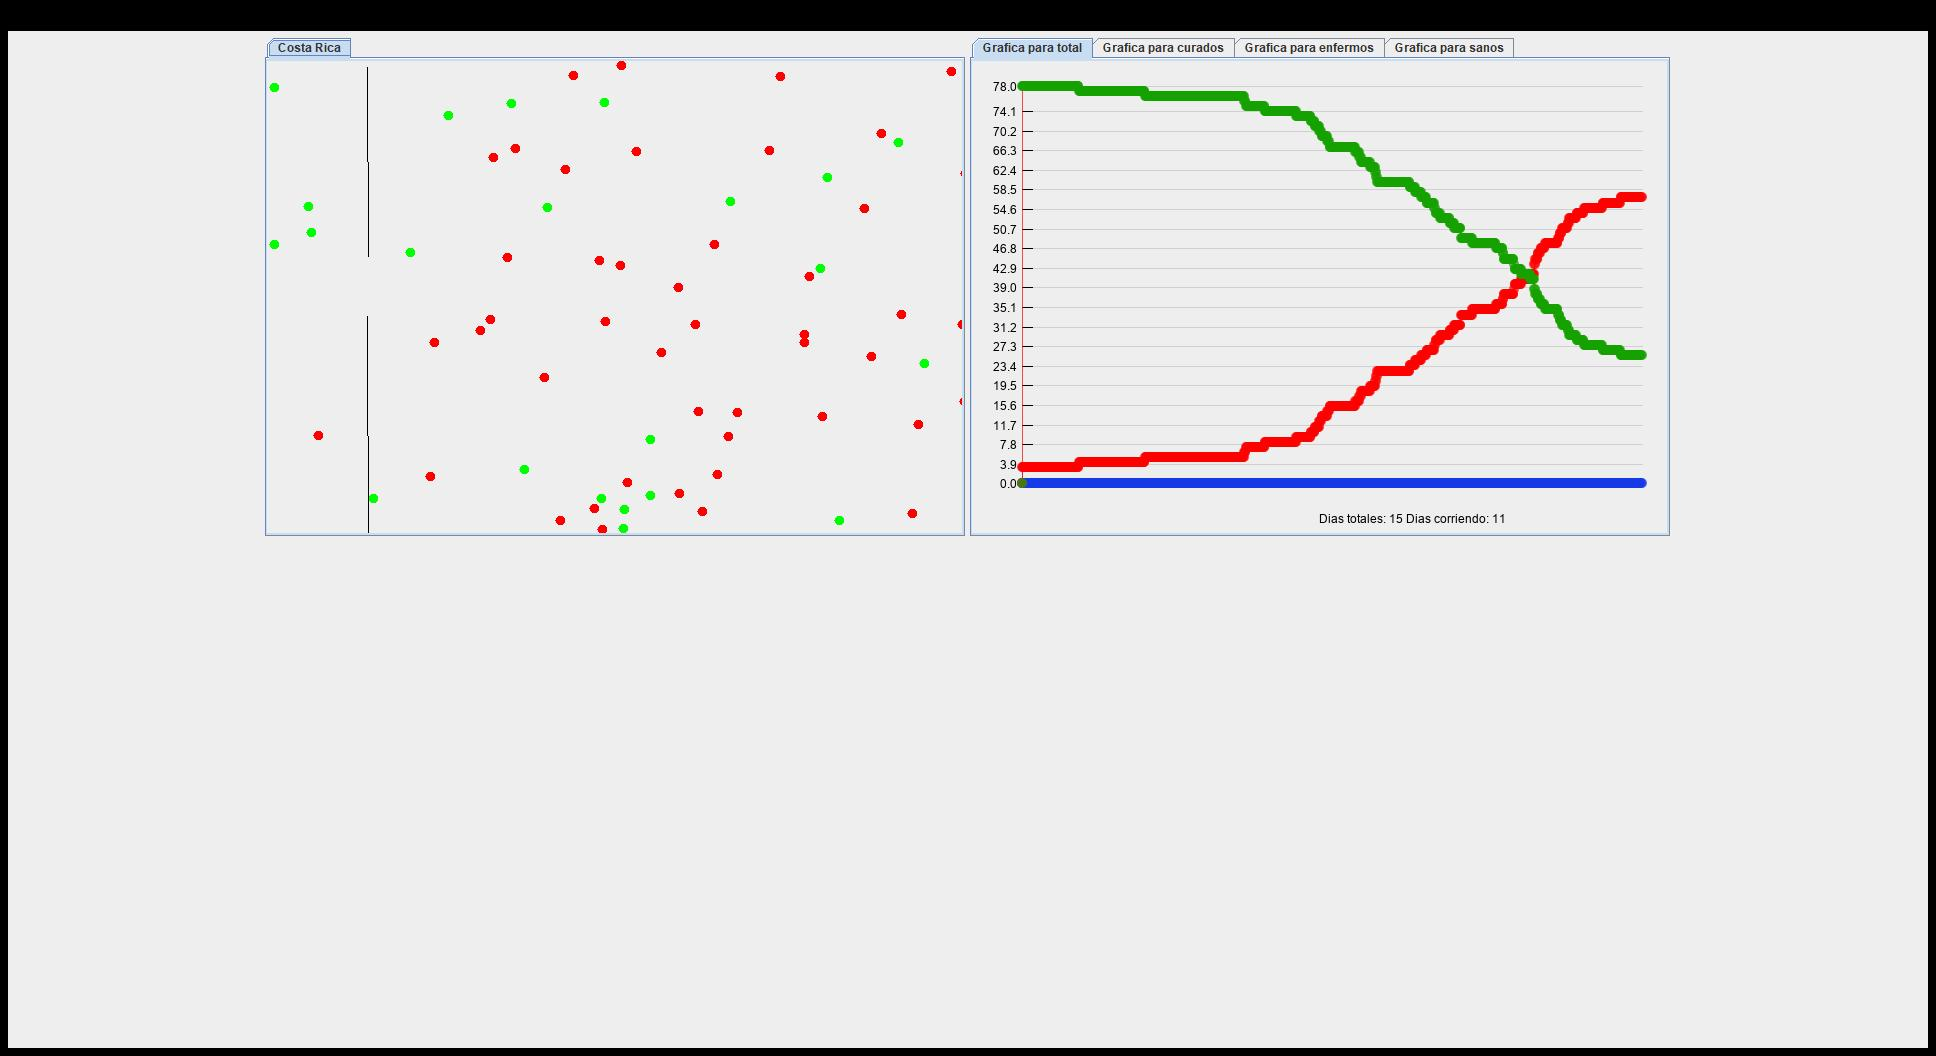
\includegraphics[scale=0.20]{11}
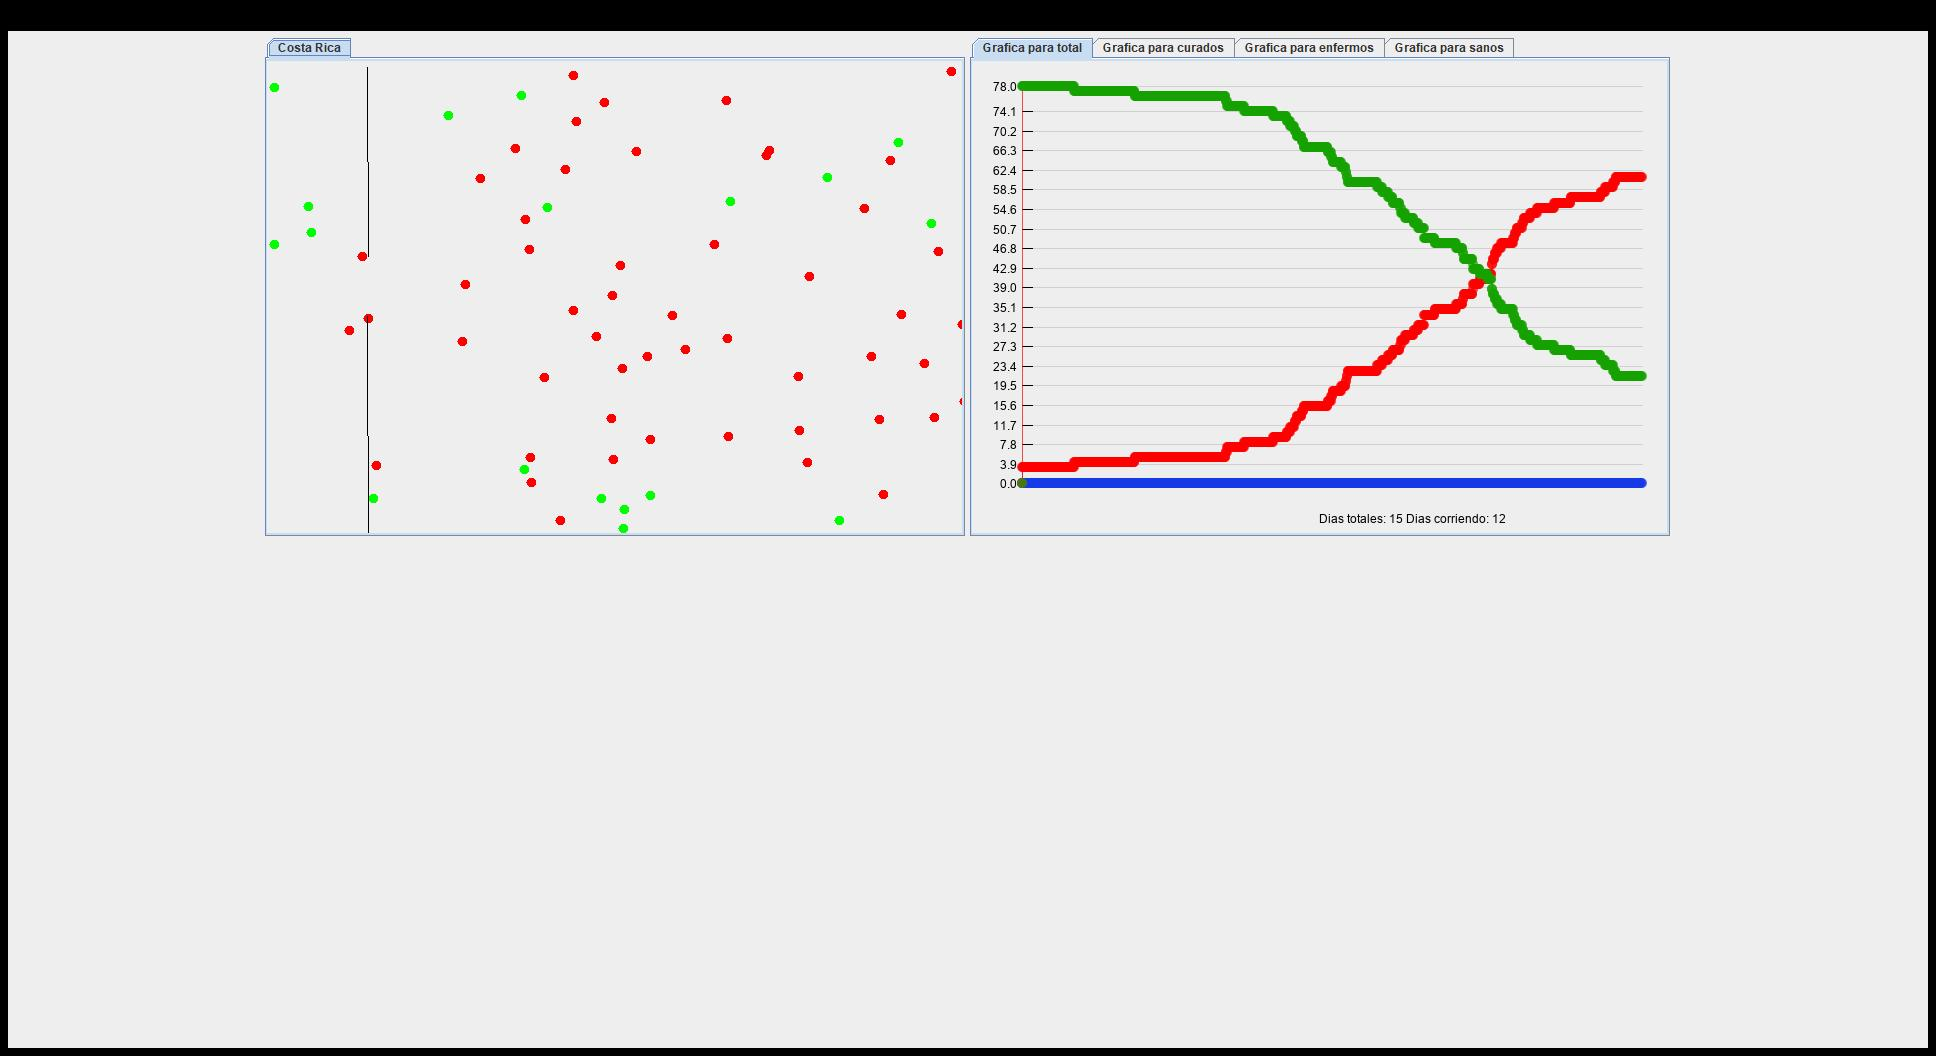
\includegraphics[scale=0.20]{12}
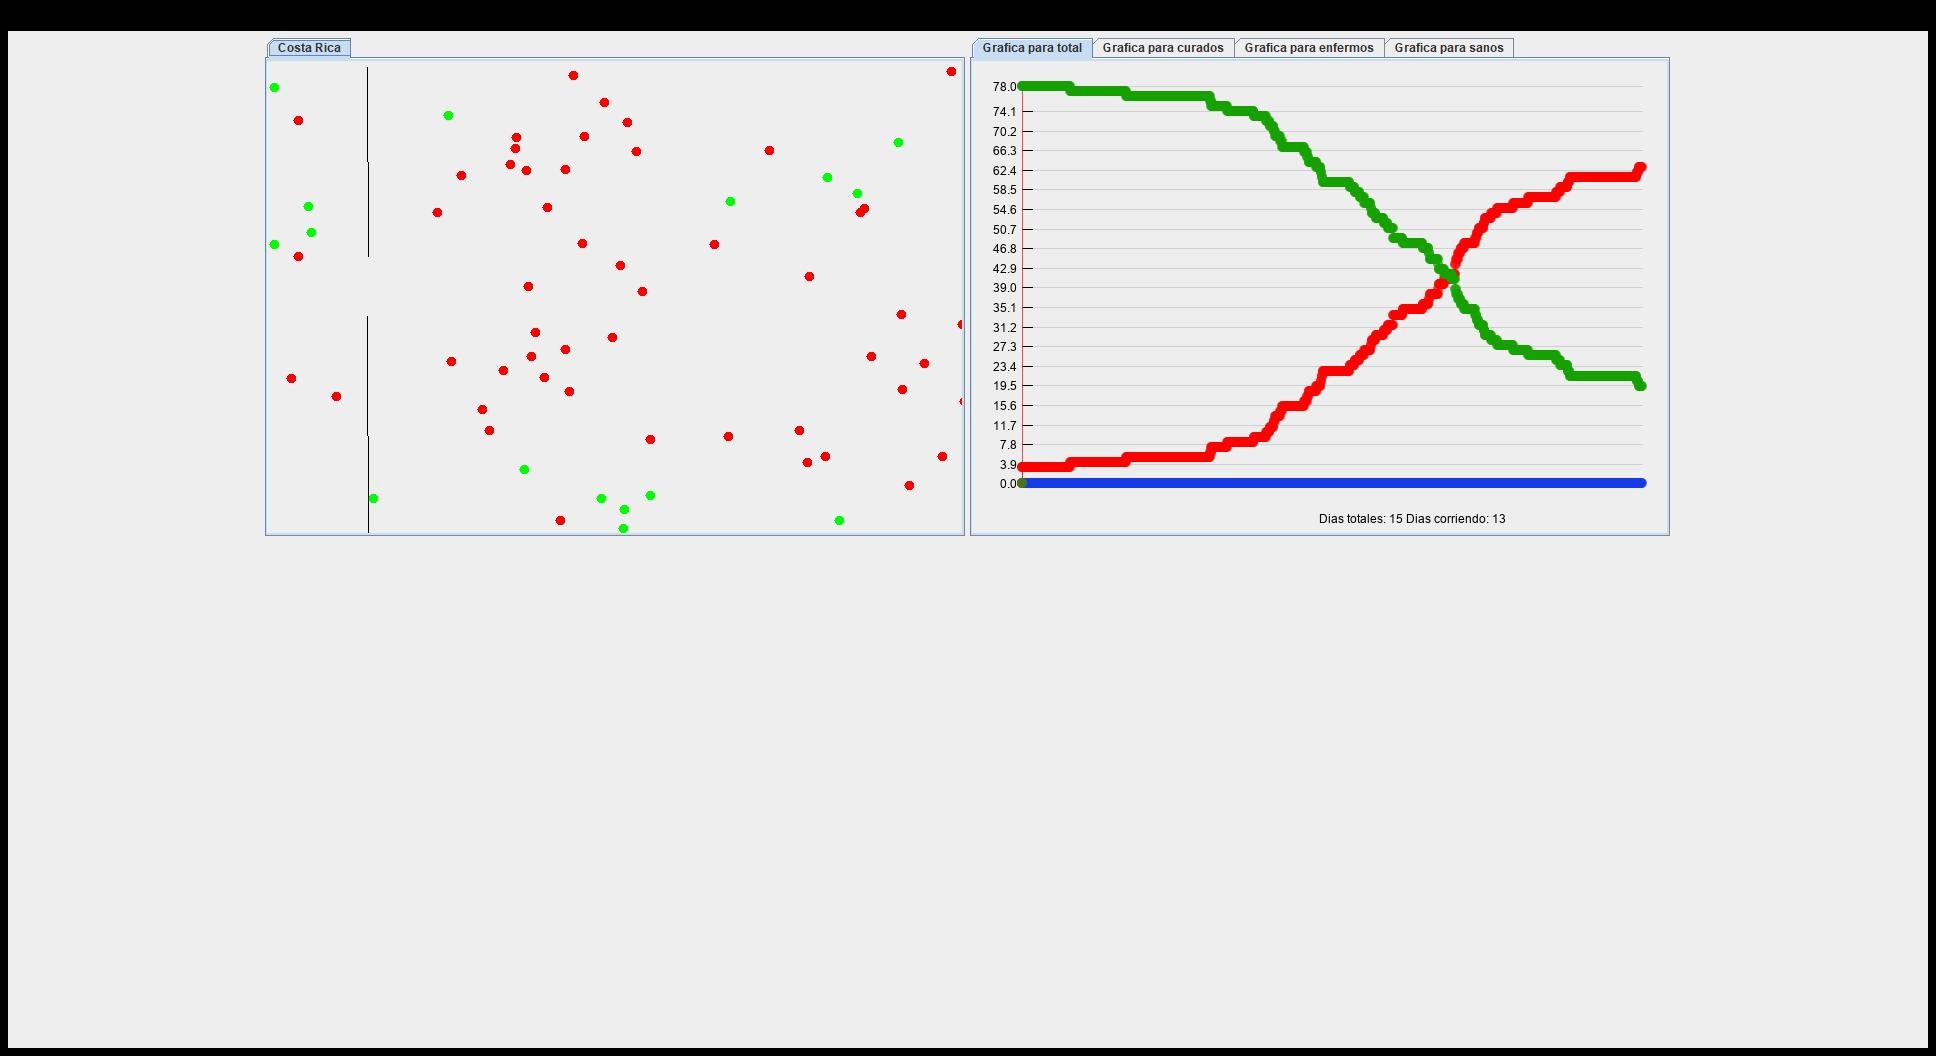
\includegraphics[scale=0.20]{13}
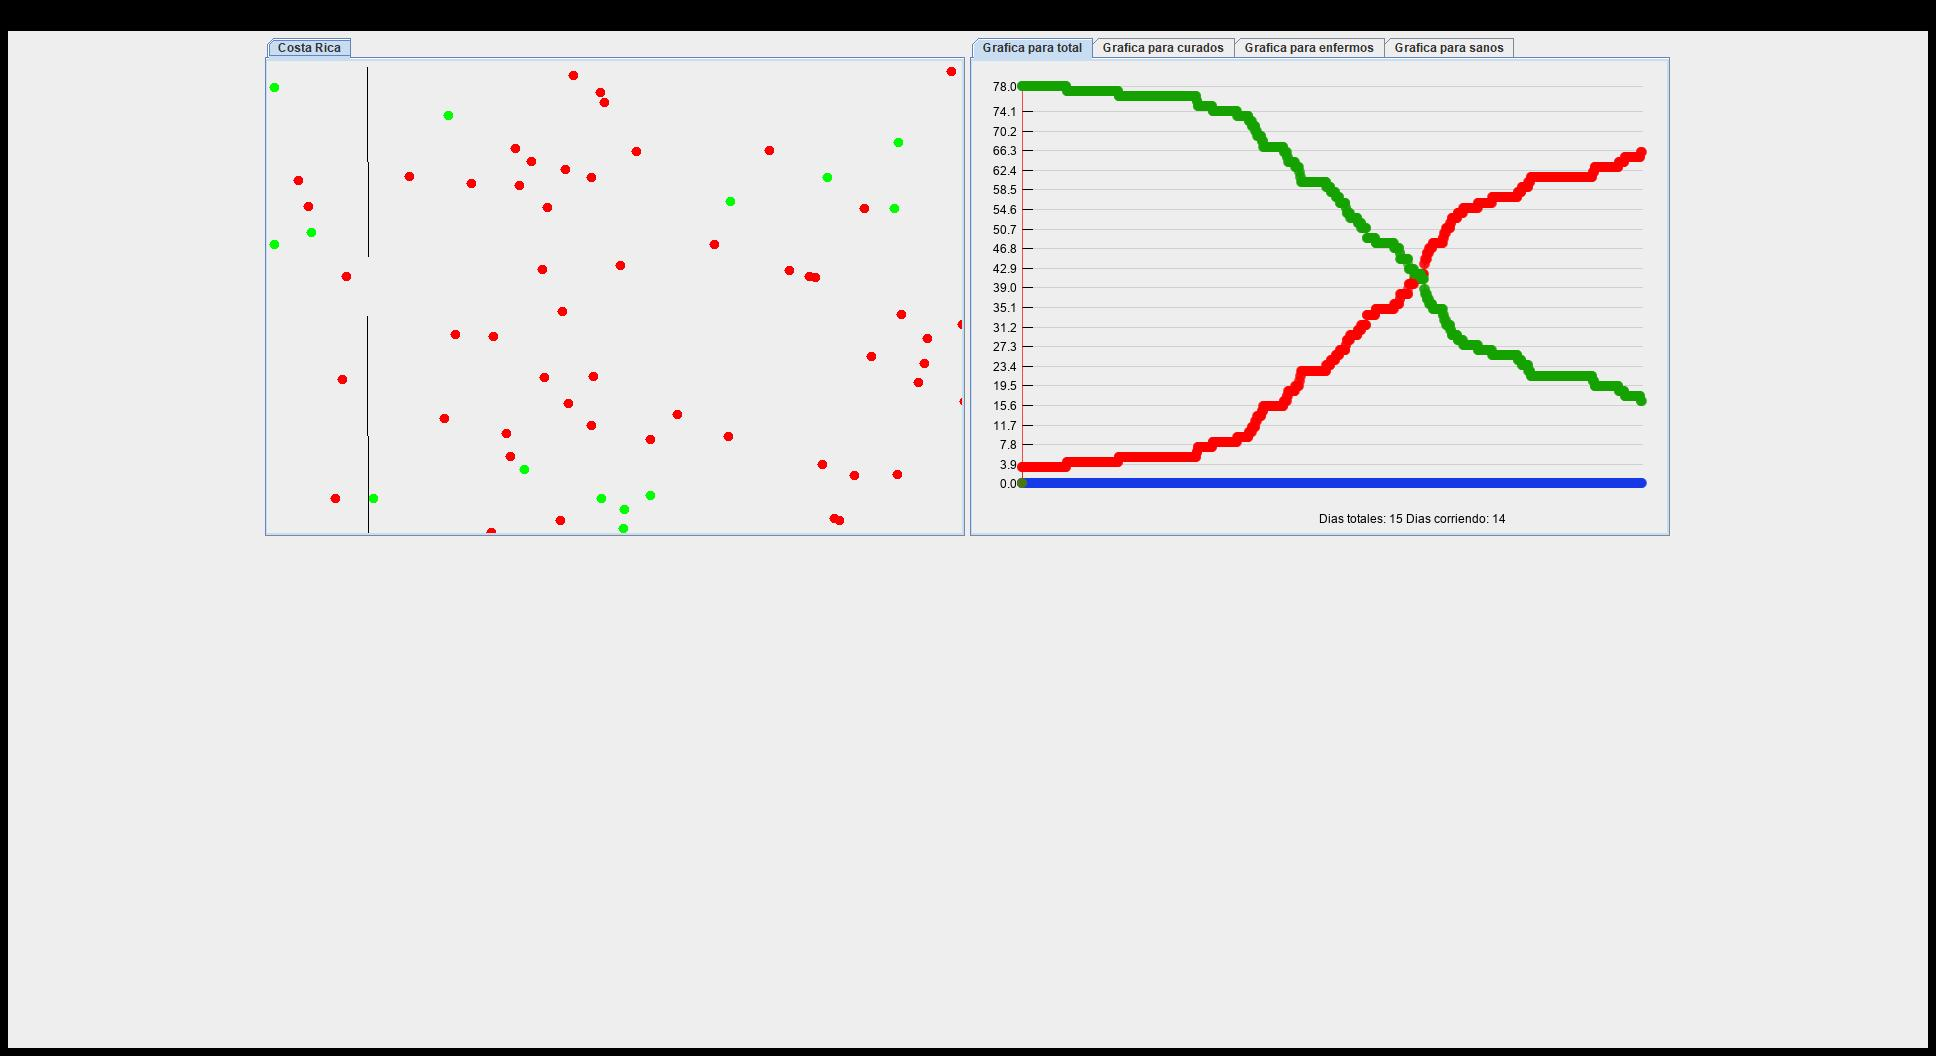
\includegraphics[scale=0.20]{14}
\end{document}
